% !TEX program = xelatex
% !TEX encoding = UTF-8 Unicode
% !TEX spellcheck = de_DE
% 
% © 2016 Moritz Brinkmann, CC-by-sa
% http://latexkurs.github.io

\documentclass[
	vorläufig=false,
	datum=2016-10-28,
	titel={Allgemeine Formatierung und Pakete},
	web=false,
]{../tex/latexkurs-slides}


\begin{document}
\begin{frame}{Übersicht}
	\tableofcontents
\end{frame}

\section{Engines und Formate}
\begin{frame}{\TeX-Engines und -Formate}{Begriffsbildung}
	\begin{description}
		\item[engine] Das Programm, das die eigentliche Satz-Arbeit macht:\\\TeX, \hologo{pdfTeX}, \luaTeX
		\item[format] Große Sammlung von Makros, die die Arbeit erleichtern sollen:\\plain\TeX, \LaTeX, \hologo{ConTeXt}
		\item[distribution] Bundle von Engines, Formaten, Erweiterungen (Paketen, Modulen) und Hilfsprogrammen:\\\TeXlive, Mac\TeX, \MikTeX
	\end{description}
\end{frame}

\begin{frame}{\TeX-Engines und -Formate}{Wichtige Engines}
	\begin{description}
		\item[\TeX] Das ursprüngliche, von Donald E. Knuth geschriebene Programm.
		\item[\hologo{pdfTeX}] Engine, die direkt PDF-Dateien schreiben kann\\Ermöglicht viele PDF-spezifische Features wie z.\,B. Mikrotypografie.
		\item[\XeTeX] Verarbeitet standardmäßig utf8-Encoding, bietet die Möglichkeit, Systemschriften zu benutzen und die Textrichtung einfach zu ändern.
		\item[\luaTeX] Bietet quasi alles was \XeTeX kann und enthält die Skriptsprache Lua, die man aus dem \TeX-Dokument heraus aufrufen kann.
	\end{description}
\end{frame}

\begin{frame}[fragile]{\TeX-Engines und -Formate}{Programm\/namen}
	Ausgeführtes Programm bestimmt Engine und Format:\\[1em]
	\begin{description}
		\item[|pdftex|] \hologo{pdfTeX}-Engine, plain-Format
		\item[|pdflatex|] \hologo{pdfTeX}-Engine, \LaTeXe-Format
		\item[|latex|] \hologo{pdfTeX}-Engine, \LaTeXe-Format, DVI-Output
		\item[|xelatex|] \XeTeX-Engine, \LaTeXe-Format
		\item[|lualatex|] \luaTeX-Engine, \LaTeXe-Format, PDF-Output
	\end{description}
\end{frame}

\section{Makrotypografie}
\frame{\centering\alert{Teil II}\\\huge Makrotypografie}

\begin{frame}{Makrotypografie}
	\begin{itemize}
		\item Satzspiegel
		\item Kopf und Fußzeilen
		\item Wahl der Schriften
		\item Formatierung von Abständen
		\item Aussehen von Verzeichnissen, Fußnoten, …
	\end{itemize}
\end{frame}

\subsection{Der Satzspiegel}
\begin{frame}{Der Satzspiegel}
	Mit Satzspiegel bezeichnet man die vom Text bedeckte Fläche (im Gegensatz zu den Rändern)
	\begin{itemize}
		\item Ein- oder zweiseitiger Satz?
		\item Schriftgröße, Laufweite,
		\item Kopf- und Fußzeilen
		\item Textspalten
	\end{itemize}
\end{frame}


\begin{frame}{Klassische Satzspiegelkonstruktion}
	\centering \small
	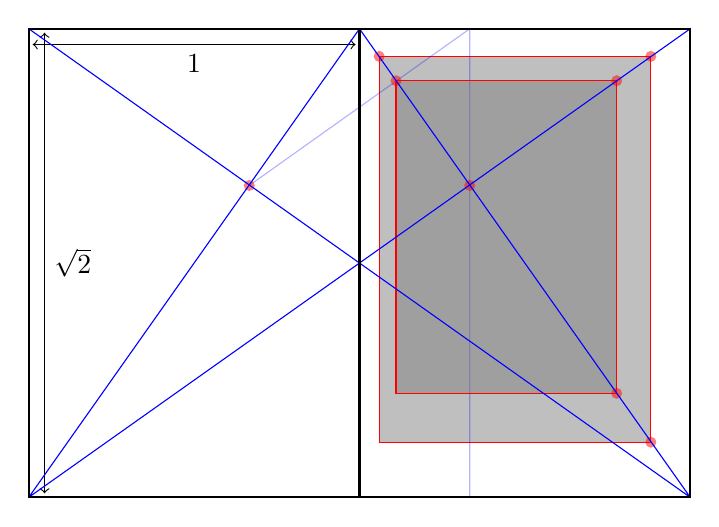
\begin{tikzpicture}
		\coordinate (a) at (-4.20, 5.95);
		\coordinate (b) at ( 0.00, 5.95);
		\coordinate (c) at ( 4.20, 5.95);
		\coordinate (d) at (-4.20, 0.00);
		\coordinate (e) at ( 0.00, 0.00);
		\coordinate (f) at ( 4.20, 0.00);

		\coordinate (A1) at ( 0.25, 5.60);
		\coordinate (B1) at ( 3.70, 5.60);
		\coordinate (D1) at ( 3.70, 0.70);
		
		\coordinate (A2) at ( 0.464, 5.29);
		\coordinate (B2) at ( 3.266, 5.29);
		\coordinate (D2) at ( 3.266, 1.32);
		\coordinate (b’) at ( 1.40, 5.95);
		\coordinate (e’) at ( 1.40, 0.00);
		\coordinate (x)  at (-1.40, 3.96);
		\coordinate (x’) at ( 1.40, 3.96);		

		\draw<2>[<->] (-4.15, 5.75) -- (-2.10, 5.75) node[below] {$1$} -- (-0.05, 5.75);
		\draw<2>[<->] (-4.00, 5.90) -- (-4.00, 2.975) node[right] {$\sqrt2$} -- (-4.00, 0.05) {};
		
		\draw<4>[red, fill=gray, fill opacity=.5] (A1) rectangle (D1);
		\fill<4>[red, opacity=0.5] 
			(A1) circle (2pt) node {}
			(B1) circle (2pt) node {}
			(D1) circle (2pt) node {};

		\draw<5>[thin ,blue, opacity=.3]
			(b’) -- (e’)
			(b’) -- (x);
		\draw<5>[red, fill=gray, fill opacity=.5] (A2) rectangle (D2);
		\fill<5>[red, opacity=0.5] 
			(A2) circle (2pt) node {}
			(B2) circle (2pt) node {}
			(D2) circle (2pt) node {}
			(x)  circle (2pt) node {}
			(x’) circle (2pt) node {};

		\draw<3->[blue]
			(d) -- (b) -- (f)
			(a) -- (f)
			(d) -- (c);	
		\draw [thick]
			(a) rectangle (e)
			(b) rectangle (f);
	\end{tikzpicture}
\end{frame}

\begin{frame}{Satzspiegelkonstruktion mit Neunerteilung}
	\centering \small
	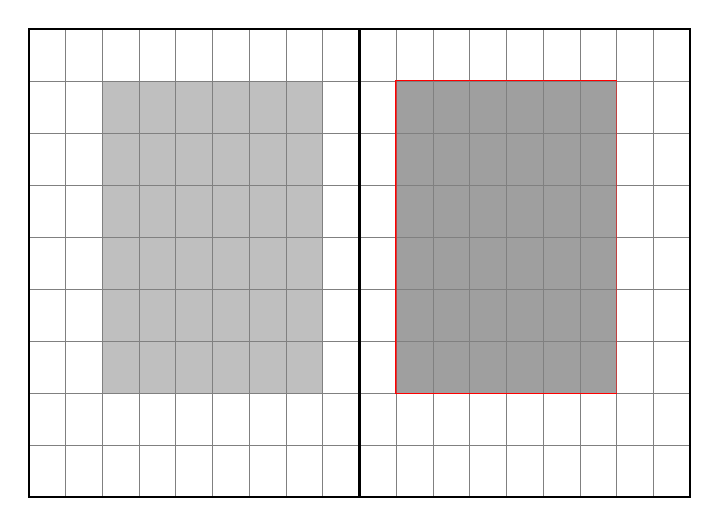
\begin{tikzpicture}
		\coordinate (a) at (-4.20, 5.95);
		\coordinate (b) at ( 0.00, 5.95);
		\coordinate (c) at ( 4.20, 5.95);
		\coordinate (d) at (-4.20, 0.00);
		\coordinate (e) at ( 0.00, 0.00);
		\coordinate (f) at ( 4.20, 0.00);
		
		\coordinate (A2) at ( 0.464, 5.29);
		\coordinate (D2) at ( 3.266, 1.32);
		\coordinate (A2’) at (-0.464, 5.29);
		\coordinate (D2’) at (-3.266, 1.32);

		\draw<1-2>[help lines, xstep=8.4/18, ystep=11.9/18] (a) grid (f);
		
		\draw<2>[red, fill=gray, fill opacity=.5] (A2) rectangle (D2);
		\fill<3>[gray, fill opacity=.5] (A2) rectangle (D2);
		\fill<3>[gray, fill opacity=.5] (A2’) rectangle (D2’);

		\draw [thick]
			(a) rectangle (e)
			(b) rectangle (f);
	\end{tikzpicture}
\end{frame}
%% Markus Kohm: „Satzspiegelkonstruktionen im Vergleich“ http://www.dante.de/tex/Dokumente/KohmSatzspiegel.pdf

\begin{frame}{Satzspiegel bei Gutenberg}
	\hspace{5.4cm}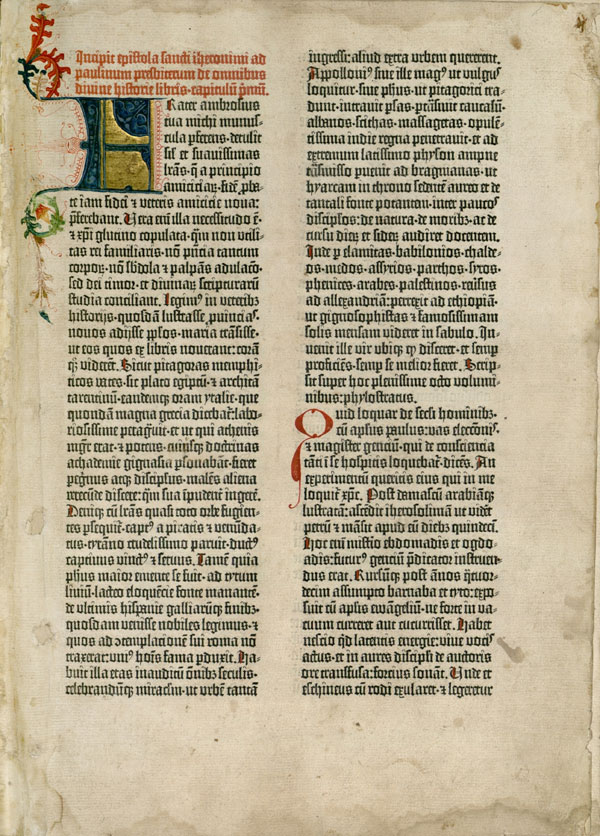
\includegraphics[height=5.95cm]{01_gutenbergbibel}
\end{frame}

\begin{frame}[fragile]{Satzspiegel mit KOMA-Skript}
\vspace{-2em}
\overleaf{tex0101}
\begin{itemize}
	\item KOMA-Skript bietet optimale Satzspiegelkonstruktion mittels eigenem Paket |typearea|
	\item Anpassung eigentlich nur bei besonders breiten oder engen Schriften nötig: Option |DIV=|\meta{Faktor}
	\\Autom. Berechnung anhand der Seitengröße: |DIV=calc| 
	\\Berechnung nach mittelalterl. Buchseitenkanon: |DIV=classic|
	\item Bindekorrektur mittels Option |BCOR=|\meta{Länge}
\end{itemize}
\begin{lstlisting}
\documentclass[DIV=9, BCOR=12mm]{scrbook}	
\end{lstlisting}
\vfill
\begin{olcol}
Bei Nicht-KOMA-Klassen muss |typearea| direkt geladen werden:
\begin{lstlisting}
\usepackage[DIV=13, BCOR=2cm]{typearea}
\end{lstlisting}
\end{olcol}
\end{frame}

\begin{frame}[fragile]{Satzspiegel mit |geometry|}\overleaf{tex0101}%
Paket |geometry|  erlaubt manuelle Einstellung des Satzspiegels:
\begin{lstlisting}
\usepackage[top=2cm, bottom=5cm]{geometry}
\end{lstlisting}
oder:
\begin{lstlisting}
\usepackage{geometry}
\geometry{top=2cm, bottom=5cm}
\end{lstlisting}
%Im Zweifelsfall besser z.\,B. auf |typearea| verlassen.
\end{frame}


\begin{frame}[fragile,t]{Satzspiegel mit |geometry|}
	\overleaf{tex0101}
	\vspace{-1.5em}
	\begin{block}{mögliche Optionen}
		\vspace{-1em}
\begin{verbatim}
paper
left, right, inner, outer, hmargin
top, bottom, vmargin
margin
bindingoffset, textwidth, textheight
twocolumn, columnsep, marginparsep, footnotesep
headsep, footsep, nofoot, nohead
hoffset, voffset, offset
\end{verbatim}
	\end{block}
\end{frame}



\subsection{Kopf- und Fußzeilen}
\begin{frame}[fragile, t]{Kopf- und Fußzeilen}
	\overleaf{tex0101}
	\begin{itemize}
		\item Kopf- und Fußzeilen enthalten wichtige Informationen über das Dokument 
		\begin{itemize}
			\item lebende Kolumnentitel
			\item Seitenzahlen
		\end{itemize}
		\item Anpassung mittels verschiedener Pakete
		\item Auswahl über |\pagestyle{|\meta{Seitenstil}|}| oder |\thispagestyle{|\meta{Seitenstil}|}| 
		\item Voreinstellungen: |empty|, |plain|, |headings|
	\end{itemize}
\end{frame}


\begin{frame}[fragile, t]{Kopf- und Fußzeilen mit fancyhdr}
	\overleaf{tex0101}
\begin{lstlisting}
\usepackage{fancyhdr}
\pagestyle{fancy}
\end{lstlisting}
	\begin{columns}
		\begin{column}{.45\textwidth}
			\vspace{-3.87em}
			
			Einseitiger Satz:
\begin{lstlisting}
\lhead{}    \lfoot{}
\chead{}    \cfoot{}
\rhead{}    \rfoot{}
\end{lstlisting}
		\end{column}
		\begin{column}{.45\textwidth}
		Zweiseitiger Satz:
\begin{lstlisting}
\fancyhead[LO]{}
\fancyhead[RO,LE]{}
\fancyhead[CE]{}
\fancyfoot[LO]{}
\fancyfoot[RO,LE]{}
\fancyfoot[CE]{}
\end{lstlisting}
		\end{column}
	\end{columns}
\end{frame}


\begin{frame}[fragile, t]{Kopf- und Fußzeilen mit scrlayer-scrpage}%
\overleaf{tex0101}%
\kern-.7ex Paket definiert zwei Seitenstile: |scrheadings| und |screadings.plain|

Anpassung mittels z.\,B.\\|\lehead[|\meta{Inhalt plain.scrheadings}|]{|\meta{Inhalt scrheadings}|}|

\begin{center}\vspace{-1em}\small
\begin{tikzpicture}
		\coordinate (a) at (-.5\textwidth, 3.50);
		\coordinate (b) at ( 0.00, 3.50);
		\coordinate (c) at ( .5\textwidth, 3.50);
		\coordinate (d) at (-.5\textwidth, 2.70);
		\coordinate (e) at ( 0.00, 2.70);
		\coordinate (f) at ( .5\textwidth, 2.70);
		\coordinate (g) at (-.5\textwidth, 0.80);
		\coordinate (h) at ( 0.00, 0.80);
		\coordinate (i) at ( .5\textwidth, 0.80);
		\coordinate (j) at (-.5\textwidth, 0.00);
		\coordinate (k) at ( 0.00, 0.00);
		\coordinate (l) at ( .5\textwidth, 0.00);

		\node (A) at (-3/8*\textwidth, 3.00) {\color{red}|\lehead|};
		\node (B) at (-2/8*\textwidth, 3.00) {\color{green}|\cehead|};
		\node (C) at (-1/8*\textwidth, 3.00) {\color{blue}|\rehead|};
		\node (D) at ( 1/8*\textwidth, 3.00) {\color{blue}|\lohead|};
		\node (E) at ( 2/8*\textwidth, 3.00) {\color{green}|\cohead|};
		\node (F) at ( 3/8*\textwidth, 3.00) {\color{red}|\rohead|};
		
		\node (G) at (-3/8*\textwidth, 0.50) {\color{red}|\lefoot|};
		\node (H) at (-2/8*\textwidth, 0.50) {\color{green}|\cefoot|};
		\node (I) at (-1/8*\textwidth, 0.50) {\color{blue}|\refoot|};
		\node (J) at ( 1/8*\textwidth, 0.50) {\color{blue}|\lofoot|};
		\node (K) at ( 2/8*\textwidth, 0.50) {\color{green}|\cofoot|};
		\node (L) at ( 3/8*\textwidth, 0.50) {\color{red}|\rofoot|};

\only<2>{
		\node (M) at ( 0, 2.6) {\color{blue}\texttt{\textbackslash ihead}};
		\node (N) at ( 0, 2.3) {\color{green}\texttt{\textbackslash mhead}};
		\node (O) at ( 0, 2.0) {\color{red}\texttt{\textbackslash ohead}};
		
		\node (P) at ( 0, 0.9) {\color{blue}\texttt{\textbackslash ifoot}};
		\node (Q) at ( 0, 1.2) {\color{green}\texttt{\textbackslash mfoot}};
		\node (R) at ( 0, 1.5) {\color{red}\texttt{\textbackslash ofoot}};
		
		\draw [red, smooth, out=270, in=180] (A.south) to (O.west);
		\draw [red, smooth, out=0, in=270]	(O.east) to (F.south);
		\draw [green, smooth, out=270, in=180] (B.south) to (N.west);
		\draw [green, smooth, out=0, in=270]	(N.east) to (E.south);
		\draw [blue, smooth, out=270, in=180] (C.south) to (M.west);
		\draw [blue, smooth, out=0, in=270]	(M.east) to (D.south);
		
		\draw [red, smooth, out=90, in=180] (G.north) to (R.west);
		\draw [red, smooth, out=0, in=90]	(R.east) to (L.north);
		\draw [green, smooth, out=90, in=180] (H.north) to (Q.west);
		\draw [green, smooth, out=0, in=90]	(Q.east) to (K.north);
		\draw [blue, smooth, out=90, in=180] (I.north) to (P.west);
		\draw [blue, smooth, out=0, in=90]	(P.east) to (J.north);
}
		\draw [thick]
			(d) -- (a) -- (c) -- (f)
			(g) -- (j) -- (l) -- (i)
			(b) -- (e)
			(h) -- (k);
		\draw [thick, dashed]
			(d) -- (g)
			(f) -- (i);
		\draw<1>[thick, dashed] (e) -- (h);
\end{tikzpicture}
\end{center}\vspace{-.5em}

\begin{olcol}
\begin{lstlisting}
\documentclass{scrartcl}
\usepackage{scrlayer-scrpage}
\lohead*{Peter Musterheinzel}
\rohead*{Seitenstile mit KOMA-Script}
\pagestyle{scrheadings}
\end{lstlisting}
\end{olcol}
\end{frame}



\subsection{Umgebungen}
\begin{frame}[fragile]{Umgebungen}
\begin{itemize}
\item \LaTeX-Dokumente werden oft von Umgebungen strukturiert:
\end{itemize}

|\begin{|\meta{Umgebung}|}[|\meta{ggf. opt. Argumente}|]{|\meta{ggf. Argumente}|}|\\
\dots\\
|\end{|\meta{Umgebung}|}|

\begin{itemize}
\item Am Anfang und Ende werden Befehle ausgeführt um bestimmtes Verhalten innerhalb der Umgebung zu erreichen.\\
\item Jede Umgebnung ist eine Gruppierung (wie |{}|)\\⇒ Alle Einstellungen innerhalb einer Umgebung sind lokal.
\end{itemize}
\end{frame}

\begin{frame}[fragile]{Umgebungen}
\begin{block}{wichtige Umgebungen}
\begin{tabular}{ll}
Aufzählung & |itemize| \\
Nummerierung & |enumerate| \\
wörtliche Wiedergabe & |verbatim| \\
zweispaltiger Satz & |twocolumn|\\
Zitat & |quotation| \\
zentriert & |center|\\
abgeschlossene Einheit & |minipage|\\
Tabelle & |tabular|, |tabularx|, |tabulary|,\\
         & |supertabular| etc. \\
Abbildung & |figure| \\
Gleitumgebung & |table| \\
Beamerfolie & |frame| \\
Gleichung & |align| (Mathe)\\
Matrix & |matrix| (Mathe)\\
\end{tabular}
\end{block}
\end{frame}

\begin{frame}[fragile]{Umgebungen}{Einfache Listen}
\begin{LTXexample}
\begin{itemize}
  \item Erster Punkt
  \item Zweiter Punkt
  \item[3] Dritter Punkt
\end{itemize}
\end{LTXexample}
\begin{LTXexample}
\begin{enumerate}
  \item Erster Punkt
  \item Zweiter Punkt
  \item[3] Dritter Punkt
\end{enumerate}
\end{LTXexample}
Aussehen von |itemize| und |enumerate| wird von Dokumentenklasse bestimmt.
\end{frame}


\subsection{Schriften (und Kodierungen)}
\begin{frame}[fragile]{Eingabekodierung}
\begin{itemize}
\item Früher\texttrademark\pdfmarginpar{Früher heißt hier in den 60er und 70er Jahren.} hat man Buchstaben mit 7\,bit gespeichert\\
z.\,B. ASCII-Zeichensatz:
\begin{verbatim*}
 !"#$%&'()*+,-./0123456789:;<=>?
@ABCDEFGHIJKLMNOPQRSTUVWXYZ[\]^_
`abcdefghijklmnopqrstuvwxyz{|}~ 
\end{verbatim*}
\item<2-> \hologo{pdfLaTeX} geht von ASCII-Kodierung aus und versteht normalerweise keine Umlaute.\\
Kodierung kann mittels |\usepackage[utf8]{inputenc}| auf Unicode umgestellt werden.
\item<3-> \XeLaTeX und \hologo{LuaLaTeX} gehen von UTF8-Kodierung aus.
\end{itemize}
\end{frame}

\begin{frame}[fragile]{Ausgabekodierung}
\begin{itemize}
\item Auch wenn \hologo{pdfLaTeX} Unicode-Eingabe versteht, erscheinen in der Ausgabe nicht unbedingt Umlaute. \hfill z.\,B. ü → ¨u
\item Ausgabekodierung kann festgelegt werden mittels |\usepackage[|\meta{Kodierung}|]{fontenc}|
\item Es verschiedene Kodierungen zur Verfügung:
\\|OT1| (original \TeX-Encoding, 7\,bit), |T1| (Latein, Mitteleuropa, 8\,bit), |T2A|\,–\,|T2C| (Kyrillisch), |T3| (Phonetisches Alphabet),\\|T4| (Latein, Afrika), |T5| (Vietnamesisch), …
\end{itemize}
\begin{lstlisting}
\usepackage[T1]{fontenc}
\end{lstlisting}
\pause
\begin{itemize}
\item \XeLaTeX und \hologo{LuaLaTeX} nutzen intern automatisch |EU1|- bzw. |EU2|-Kodierung (Unicode). |T1| muss  nur bei Verwendung von \hologo{pdfLaTeX}-Schriften explizit angegeben werden.
\end{itemize}
\end{frame}

\begin{frame}[fragile,t]{Schriften in \hologo{pdfLaTeX}}
\overleaf{tex0102}
\begin{itemize}
\item \hologo{pdfLaTeX} benötigt bestimmtes Schriftformat (\TeX{} font metrics)
\item Schriften werden mittels Paketen geladen.
\end{itemize}
\begin{lstlisting}
\usepackage{kpfonts}
\end{lstlisting}
\begin{itemize}
\item In \href{http://www.ctan.org}{CTAN}\pdfmarginpar{Comprehensive TeX Archive Network ist ein Umfassendes Verzeichnis von (La)TeX-Paketen. http://www.ctan.org} verfügbare Schriften findet man z.\,B. im \href{http://www.tug.dk/FontCatalogue/}{„LaTeX Font Catalogue“}\\\url{http://www.tug.dk/FontCatalogue/}
\end{itemize}
\end{frame}

\begin{frame}[fragile,t]{Schriften in \XeLaTeX und \hologo{LuaLaTeX}}
\begin{itemize}
\item Paket |fontspec| erlaubt es auf Systemschriften (OTF, AAT, TTF) zuzugreifen.
\item Fonts werden über spezielle Befehle geladen |\setmainfont[|\meta{Optionen}|]{|\meta{Name der Schrift}|}|
\end{itemize}
\begin{lstlisting}
\setromanfont{Linux Libertine O}
\setsansfont{Linux Biolinum O}
\setmonofont[Scale=.95]{DejaVu Sans Mono}
\end{lstlisting}
\begin{olcol}
\begin{itemize}
\item Laden bestimmter Schriften oder Features im Dokument mit\\|\fontspec{|\meta{Name der Schrift}|}[|\meta{Features}|]|
\end{itemize}
\end{olcol}
\end{frame}

\begin{frame}[fragile]{Schriftgröße}%
\kern-0.4exDie Größe der Brotschrift kann durch Klassenoption geändert werden:
\begin{lstlisting}
\documentclass[12pt]{scrartcl}
\end{lstlisting}
Größe von |\large|, |\small|, etc. passt sich automatisch an.\\
Standardklassen unterstützen |10pt|, |11pt| und |12pt|.
\vfill
\pause
Wer \emph{genau weiß}, was er will: |\fontsize{|\meta{Größe}|}{|\meta{Durchschuss}|}\selectfont|
\begin{lstlisting}
\fontsize{10}{12}\selectfont
\end{lstlisting}
\end{frame}

\section{Mikrotypografie}
\frame{\centering\alert{Teil III}\\\huge Mikrotypografie}
\begin{frame}[t]{Mikrotypografie}
	Mikrotypografie bezeichnet die Gestaltung von Feinheiten auf Buchstabenebene:
	\begin{columns}
		\begin{column}{.65\textwidth}
%			\setlength{\labelwidth}{5cm}
			\begin{description}
				\item<1->[tracking] Anpassung des Glyphenabstands innerhalb der Wörter (≤\,3\%)
				\item<2->[expansion] Anpassung der Glyphenbreite (≤\,2\%)
				\item<3->[protrusion] Optischer Randausgleich
				\item<4->[ligatures] Verbindung mehrerer Buchstaben zu einer Glyphe
			\end{description}
		\end{column}
		\begin{column}{.25\textwidth}%
			\centering\rmfamily\Large\noindent%
			\only<1>{\LARGE\hfill V\kern1pt A\hfill F\kern1.1pt o\hfill\,\\\hfill VA\hfill Fo\hfill}%
			\only<2>{Text\\\scalebox{.98}{Text}}%
			\only<3>{\tiny\parbox{\textwidth}{Lorem ipsum dolor sit amet\textcolor{red}{,} consectetur adipisici elit, sed ei\textcolor{red}{\-}usmod tempor incidunt ut labo\textcolor{red}{\-}re et dolore magna aliqua. Ut enim ad minim veniam, quis no\textcolor{red}{\-}strud exercitation ullamco labo\textcolor{red}{\-}ris nisi ut aliquid ex ea commodi consequat. Quis aute iure repre\textcolor{red}{\-}henderit in voluptate velit esse cillum dolore eu fugiat nulla pa\textcolor{red}{\-}riatur. Excepteur sint obcaecat cupiditat non proident, sunt in culpa qui officia deserunt mollit anim id est laborum.}}%
			\only<4>{f\/i fi\\
				f\/l fl\\
				f\/f ff\\
				f\/f\/l ffl\\
				Q\/u Qu\\
			}
		\end{column}
	\end{columns}
\end{frame}

\begin{frame}[fragile]{Mikrotypografie}
Das Paket |microtype| kümmert sich um diese typografischen Feinheiten.\\
In der Regel reicht die Voreinstellung:
\begin{lstlisting}
\usepackage{microtype}
\end{lstlisting}
\begin{itemize}
\item Aktiviert automatisch protrusion (in \hologo{pdfTeX}, \XeTeX und \hologo{LuaTeX}) und expansion (in \hologo{pdfTeX} und \hologo{LuaTeX}) 
\item Für weitere Optionen: Dokumentation
\end{itemize}
\end{frame}

\begin{frame}[fragile]{Leerräume und Striche}
	Gute Typografie unterscheidet zwischen verschieden breiten Leerzeichen und horizontalen Strichen
			\begin{itemize}
				\item normales Leerzeichen
				\item schmales Leerzeichen (Spatium): |\,| \hfill z. B.\quad z.\,B.\quad z.B.
				\item kleiner Abstand (Halbgeviert): |\enskip| \hfill a\enskip b
				\item weißes Quadrat (Geviert): |\quad| \hfill a\quad b
				\item negativer Abstand: |\!| \hfill a\!b
				\pause
				\item explizites Ändern des Abstands (Kerning): |a\kern-.1em b| \hfill a\kern-.1em b
				\item[] \pause
				\item Viertelgeviertstrich, Bindestrich: |-| \hfill a-b
				\item Halbgeviertstrich, Gedankenstrich: |--| \hfill a–b
				\item Geviertstrich, engl. Gedankenstrich: |---| \hfill a—b
				\item Minuszeichen: |$-$| \hfill $a-b$\\\hfill $a+b$
			\end{itemize}
\end{frame}

\section{Sprachen}
\frame{\centering\alert{Teil IV}\\\huge Sprachen, Dokumentation \& Fehlermeldungen}
\begin{frame}[fragile]{Sprachen}
Dokument muss je nach Eingabesprache lokalisiert werden.
\begin{itemize}
	\item Umbruchregeln
	\item Bezeichnungen von Verzeichnissen, Kapiteln, …
	\item typografische Besonderheiten
\end{itemize}
\begin{lstlisting}
\usepackage[ngerman]{babel}
\end{lstlisting}
%Umstellen der Sprache mittels\\
%|\selectlanguage{|\meta{Sprache}|}|
%|\foreignlanguage{|\meta{Sprache}|}{|\meta{Text}|}|
%|\begin{otherlanguage}{|\meta{Sprache}|}|\\
%|\end{otherlanguage}|
\pause
\vfill
Modernere Alternative für \hologo{LuaLaTeX} und \XeLaTeX:
\begin{lstlisting}
\usepackage{polyglossia}
\setmainlanguage{german}
\end{lstlisting}
%\setotherlanguage{english}
\end{frame}


\begin{frame}[fragile]{Standardpakete}
\hologo{pdfLaTeX}
\begin{lstlisting}
\usepackage[ngerman]{babel}
\usepackage[T1]{fontenc}
\usepackage[utf8]{inputenc}
\end{lstlisting}
\vfill
\XeLaTeX \pdfmarginpar{Das Paket xltxtra läd neben einigen XeTeX-spezifischen Definitionen fontspec automatisch, sodass fontspec hier nicht separat aufgerufen werden muss.}
\begin{lstlisting}
\usepackage{polyglossia}
\setmainlanguage{german}
\usepackage{xltxtra}
\end{lstlisting}
\vfill
\hologo{LuaLaTeX}
\begin{lstlisting}
\usepackage{fontspec}
\usepackage{polyglossia}
\setmainlanguage{german}
\end{lstlisting}
\end{frame}

\section{Dokumentation}
\begin{frame}{Dokumentation}
	\begin{itemize}
		\item \hologo{LaTeXTeX} ist hervorragend dokumentiert
		\item Jede Klasse und jedes Paket bringt normalerseise eine eigene Anleitung mit.
		\item Dokumentation kann mittels des \texttt{texdoc}-Befehls aufgerufen werden
	\end{itemize}
\end{frame}

\begin{frame}[fragile]{Dokumentation}
	Auf der Kommandozeile:
	\begin{itemize}
		\item |texdoc| durchsucht die \LaTeX-Ordner nach Dokumentationen
		\item |texdox amsmath| öffnet |amsmath.pdf|
		\item |texdoc -l amsmath| listet alle Ergebnisse auf
		\item |texdoc -s amsmath| liefert Ergebnisse aus erweiterter Suche
		\item |texdoc --help| zeigt eine Hilfe an
	\end{itemize}
	Mit |texdoctk| existiert eine grafische Oberfläche
\end{frame}

\section{Fehlermeldungen}
\begin{frame}[t]{Umgang mit Fehlern}
	\begin{block}{Was tun, wenn \LaTeX anhält?}
		\begin{itemize}
			\item Ruhe bewahren! (\texttt{tex}-Dateien können nicht beschädigt werden)
			\item Mit der Fehlersuche beim den letzten Änderungen anfangen.
			\item Ggf. Schreibfehler korrigieren.
			\item \texttt{log}-Datei Lesen!
			\item Viele Editoren helfen bei der Fehlersuche, indem sie zur Zeile springen, in der der Fehler aufgetreten ist. (Das muss nicht die fehlerhafte Zeile sein.)
		\end{itemize}
	\end{block}
\end{frame}

\begin{frame}[fragile,t]{Fehlermeldungen}
Typische Fehlermeldung:
\begin{lstlisting}
! Undefined control sequence.
l.3 Ein \Latex-Dokument
                           .
? 
! Emergency stop.
l.3 Ein \Latex-Dokument.
                           .
No pages of output.
Transcript written on document.log.
\end{lstlisting}
⇒ Befehl in Zeile 3 falsch geschrieben
\end{frame}

\begin{frame}[fragile,t]{Fehlermeldungen}
Typische Fehlermeldung:
\begin{lstlisting}
Runaway argument?
{itemize \item Erstes Item 
! Paragraph ended before \begin was complete.
<to be read again> 
                   \par 
l.60 
     
? 
\end{lstlisting}
⇒ Irgendwo nach itemize ein |}| oder ein |\end{}| vergessen.
\end{frame}

\begin{frame}{Vollständiges Minimalbeispiel}
Bei Hilfestellung in Webforen/Usenet wird in der Regel ein \emph{vollständiges Minimalbeispiel} (MWE) verlangt.
\vskip1ex
\begin{enumerate}
\item solange Code aus dem Dokument löschen, bis der Fehler gerade noch auftritt
\item alle überflüssigen Pakete entfernen
\item falls Dokumentenklasse keine Rolle spielt, \pkg{minimal} verwenden
\item wenn Fehler nur bei viel Text auftritt, \pkg{blindtext} verwenden
\end{enumerate}

\vskip1ex

Oft findet man den Fehler beim erstellen des MWE schon ganz alleine.
\end{frame}

\nocite{kohm:satzspiegel, microtype, detailtypo, bringhurst}
\begin{frame}[allowframebreaks]{Weiterführende Literatur}
\printbibliography
\end{frame}


\end{document}
